\section{Object detection with YOLOv8}
\label{sec:yolo}

The third learned formulation treats lunar features as objects to be localised with bounding boxes. YOLO \citep{redmon2016yolo} frames detection as a single regression pass --- box coordinates and class probabilities are predicted simultaneously in one forward pass, avoiding the region-proposal stage of two-stage detectors and making the method orders of magnitude faster. We use YOLOv8n \citep{jocher2023yolov8} (3.0M parameters, anchor-free decoupled head), COCO-pretrained and fine-tuned on the lunar tiles. Box targets are generated from the semantic mask channels by connected-component labelling, with per-class size gates discarding degenerate components (minimum side 5\,px; maximum side 100\,px for craters, 300\,px otherwise).

\paragraph{Experiment 1: all seven classes.}
The box-level class distribution is even more skewed than the pixel-level one: impact craters contribute 382{,}122 of 399{,}691 instances (95.5\%), wrinkle ridges 16{,}133 (4.0\%), and the remaining five classes below 0.2\% each, with all boxes small relative to the image (most spanning ${\sim}5\%$ of its side). Trained for 100 epochs on this dataset, the model converges stably (a transient loss spike near epoch 90 is the cosine-annealing restart) but fails to generalise beyond the dominant class: recall grows only to ${\sim}0.05$, concentrated on craters.

\paragraph{Experiment 2: craters removed.}
Excluding the impact-crater class leaves 17{,}486 instances dominated by wrinkle ridges (92.6\%). Training on this reduced six-class dataset is markedly more stable --- all losses decrease smoothly, training and validation remain closely aligned, and recall (${\sim}0.043$) is now spread across the six rare classes rather than concentrated on craters. Class imbalance, not model capacity, was the primary limiting factor of the first experiment; even a simple class-removal curation significantly improves convergence.

\subsection{A decoupled per-group ensemble}
\label{sec:yolo_ensemble}

The natural next step is to decouple the problem entirely: instead of one seven-class model, a small ensemble of specialised detectors, each trained only on morphologically similar classes so that high-frequency features cannot overwhelm the gradient signal of rare ones. Classes are grouped by geometry --- a two-dimensional (areal) group $f_1$ (craters, pits, mare patches, Apollo sites) and a one-dimensional (curvilinear) group $f_2$ (ridges, scarps, rilles) --- and within each group the dominant class receives a dedicated single-class detector while the rest share a second one, yielding four YOLOv8n models. Figure~\ref{fig:yolo_ensemble_cm} shows the validation confusion matrices of the two multi-class members: within a morphological group the rare classes are separable once the dominant class is removed, with confusion against background as the main residual error mode.

\begin{figure}[htbp!]
\centering
\begin{subfigure}[b]{0.48\columnwidth}
    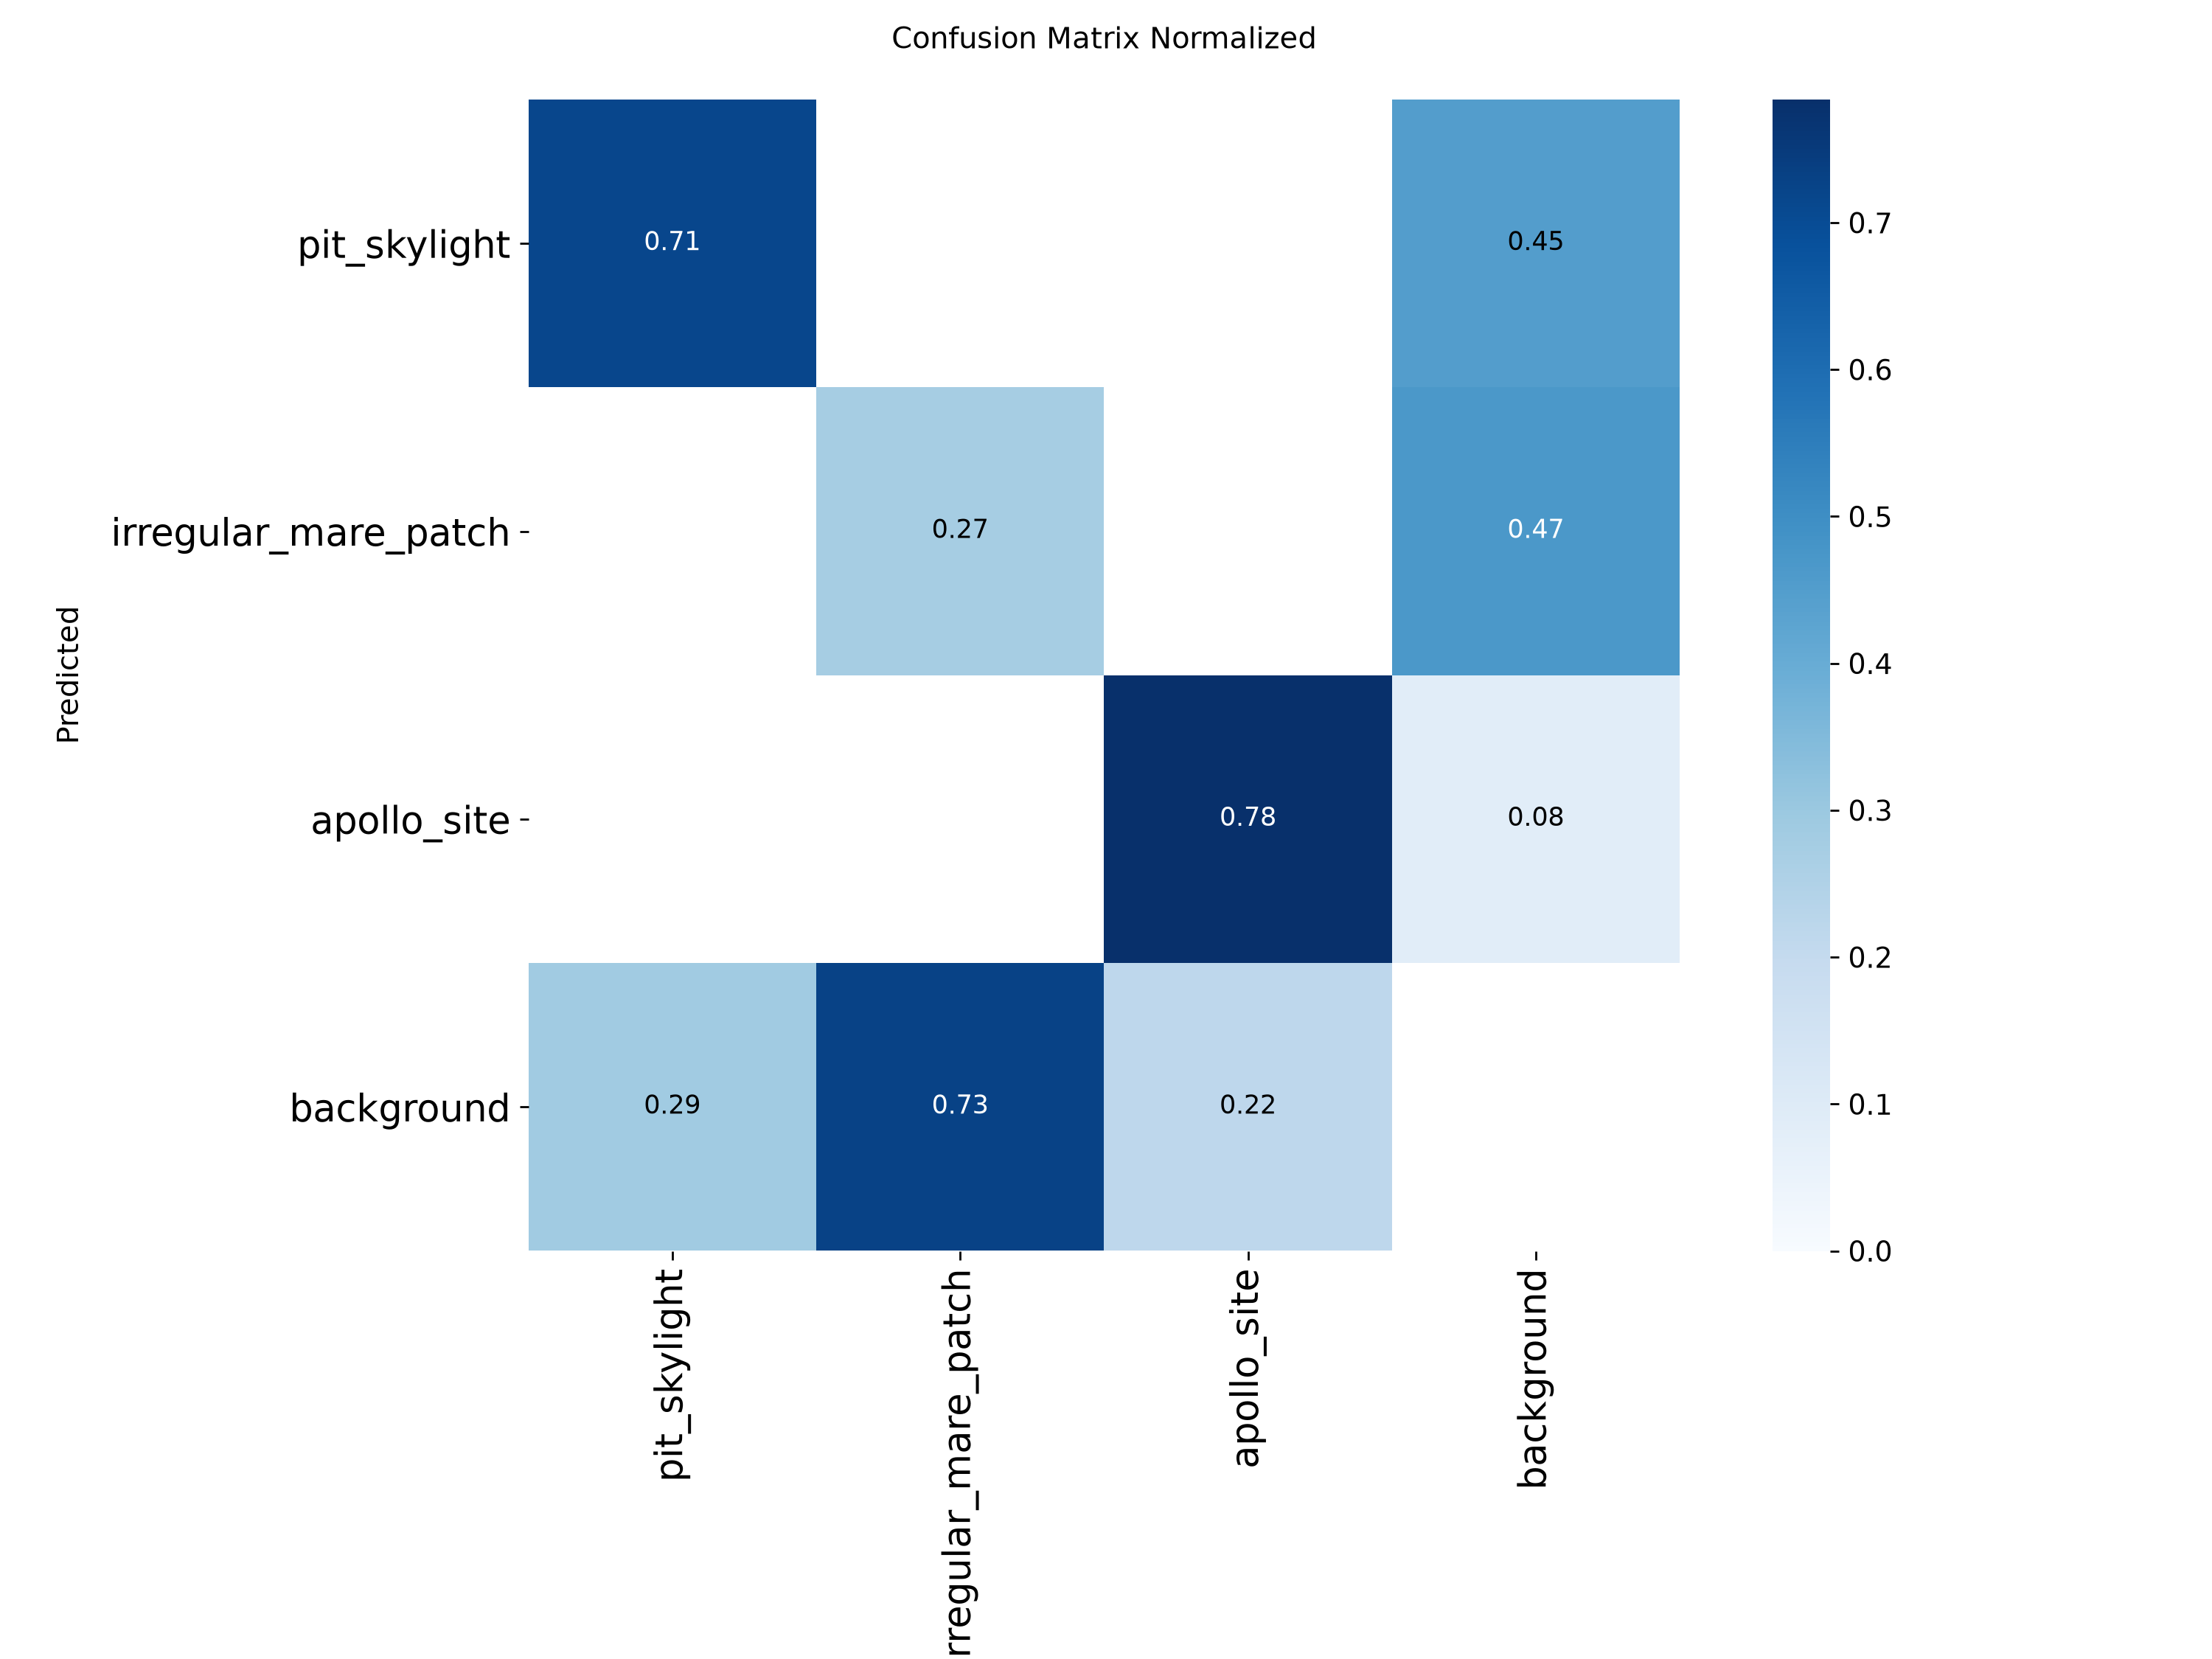
\includegraphics[width=\textwidth]{figures/YOLO/YOLO_f1.2_matrix.png}
    \caption{$f_1$ group model.}
\end{subfigure}
\hfill
\begin{subfigure}[b]{0.48\columnwidth}
    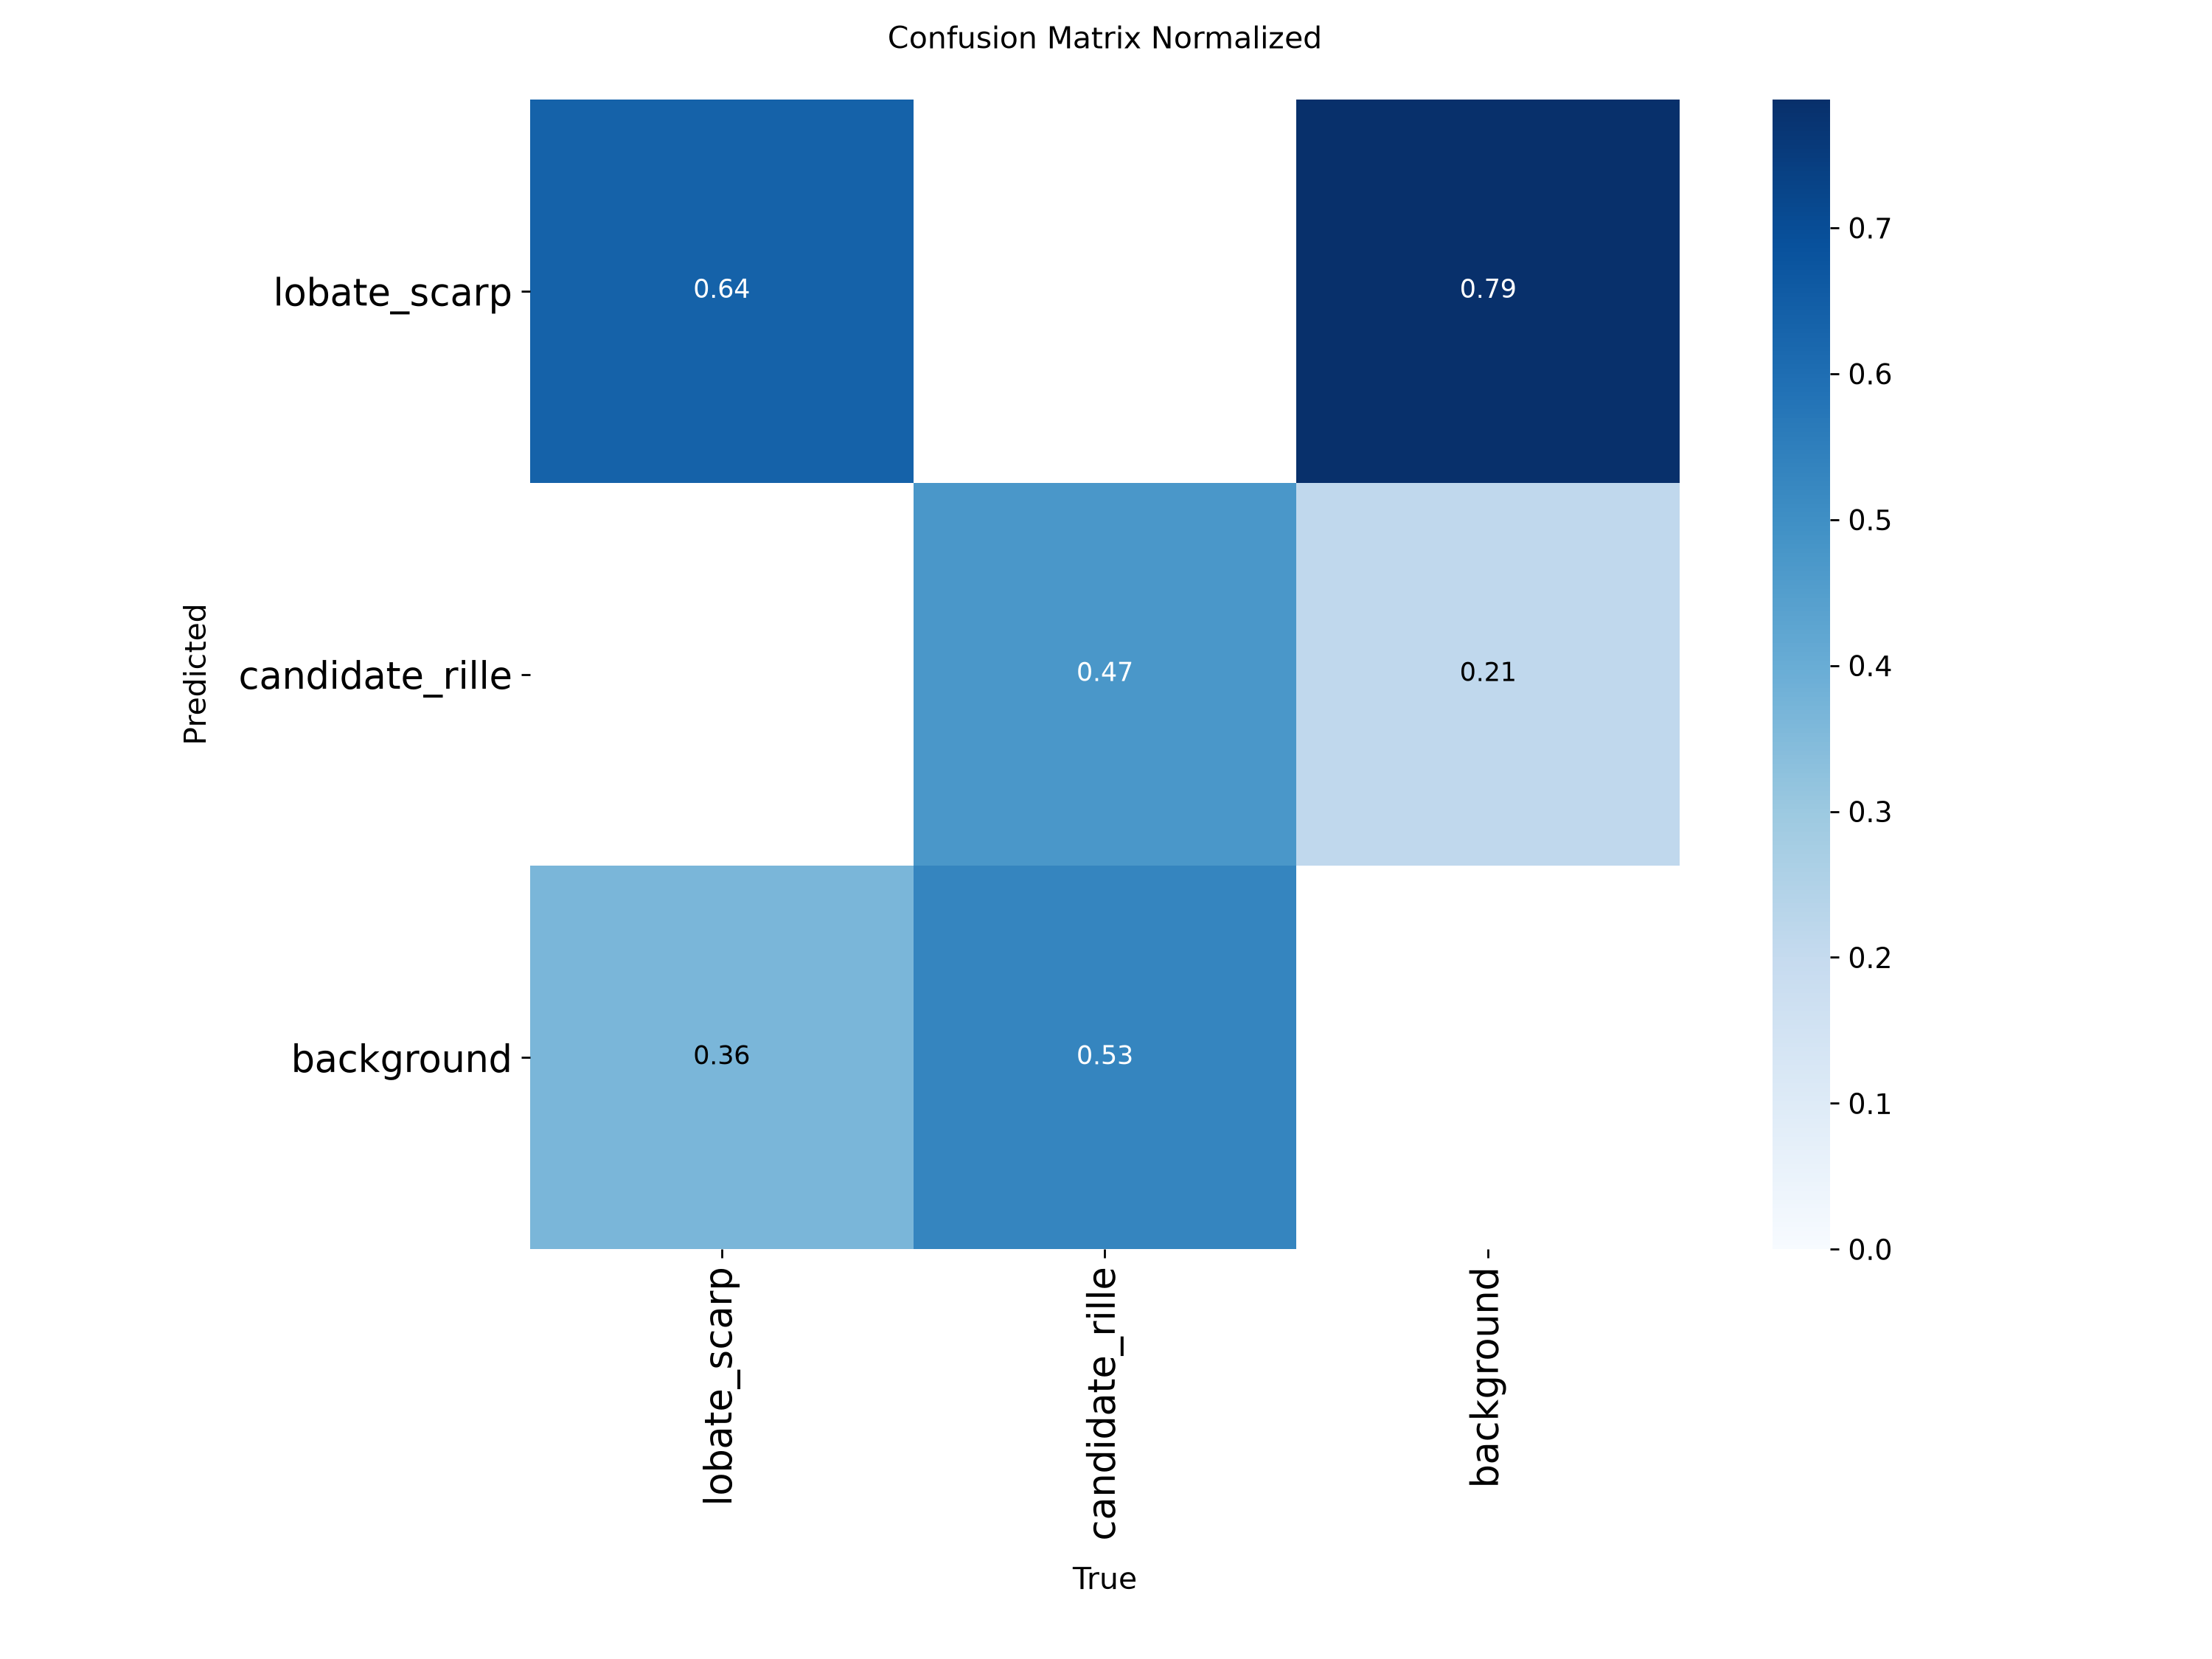
\includegraphics[width=\textwidth]{figures/YOLO/YOLO_f2.2_matrix.png}
    \caption{$f_2$ group model.}
\end{subfigure}
\caption{Normalised validation confusion matrices of the two multi-class ensemble members (random-split protocol).}
\label{fig:yolo_ensemble_cm}
\end{figure}

On the random-split protocol used during development, the training-run validation scores of the two single-class members reached mAP50 $\approx0.9$, while the multi-class members remained much lower (${\approx}0.50$ for $f_1$, ${\approx}0.25$ for $f_2$). These development scores are not comparable to the numbers of Sect.~\ref{sec:comparison}: they are measured on a random split over 50\%-overlapping tiles, on datasets restricted to feature-bearing tiles, and at a different training budget. Sect.~\ref{sec:split_study} disentangles exactly this, by retraining the ensemble's two single-class detectors under both split protocols at matched budget.
